\chapter{Configuration de la station}

\section{Création et installation de la distribution \textit{Raspbian}}

Pour une \textit{RaspberryPi}, son disque dur est nulle autre qu'une carte Micro SD. C'est donc sur ce support que nous allons faire l'installation.

Pour réaliser cette étape, vous aurez besoin de :
\begin{itemize}
	\item d'une \textit{RaspberryPi}
	\item d'une carte micro SD de minimum 4Go
	\item du logiciel \href{etcher.io}{Etcher}
	\item de \href{https://sourceforge.net/projects/dexterindustriesraspbianflavor/}{\textit{Raspbian}}. En réalité il s'agit d'une version modifiée par la société Dexter Industries qui est spécialisé dans l'utilisation de \textit{RaspberryPi} pour la robotique.
	\item d'un adaptateur pour relier la micro SD à votre ordinateur.
\end{itemize}\\
Nous pouvons désormais commencer l'installation de l'OS sur notre \textit{RaspberryPi}

\begin{enumerate}
	\item Connecter la micro SD sur votre ordinateur.\\
	\item Lancer le logiciel \textit{Etcher}\\
	\begin{figure}[H]
	\begin{center}
		\makebox[\textwidth]{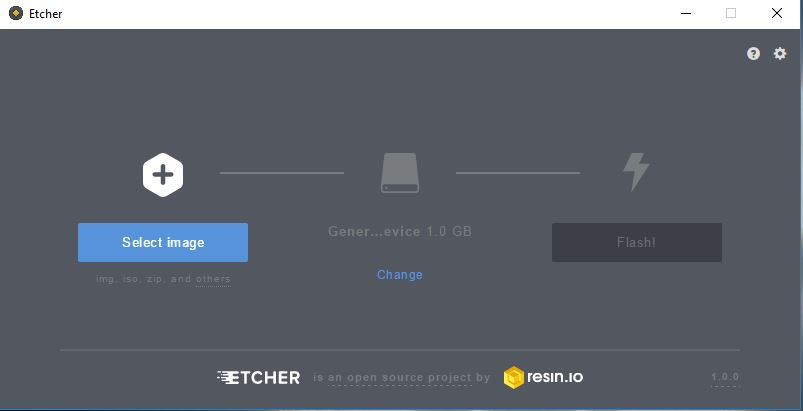
\includegraphics[width=.6\paperwidth]{images/etcher1.jpg}}
	\end{center}
		\caption{ \textit{Logiciel Etcher au lancement}}
	\end{figure}\\
	\item Cliquer sur \textit{"Select image"} à gauche puis sélectionner le fichier \textit{.zip} récupéré depuis le site \textit{SourceForce} dans les pré-requis.\\
	\item Vérifier que le périphérique qui est renseigné au centre est bien la micro SD. Dans le cas contraire cliquer sur \textit{"Change"}.\\
	\item Si les deux étapes précédentes sont OK, cliquer sur \textit{"Flash"}.\\
	\begin{figure}[H]
	\begin{center}
		\makebox[\textwidth]{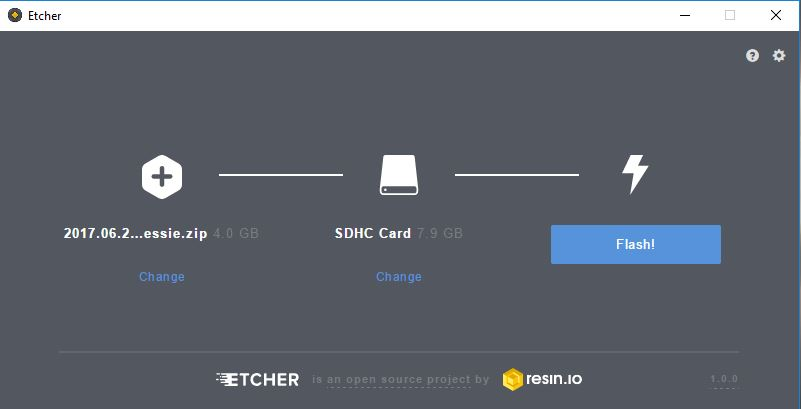
\includegraphics[width=.6\paperwidth]{images/etcher2.jpg}}
	\end{center}
		\caption{ \textit{Etcher prêt à flasher}}
	\end{figure}\\
\end{enumerate}
Et voilà, l'opération peut prendre une dizaine de minutes. C'était simple non ?

\section{Première mise en route de la \textit{RaspberryPi}}

\begin{enumerate}

	\item Maintenant que vous avez \textit{Raspbian}, nous pouvons démarrer notre nouvel ordinateur.
Pour cela, il vous suffit d'insérer la microSD au dos de la \textit{RaspberryPi}.\\
\begin{figure}[H]
\begin{center}
	\makebox[\textwidth]{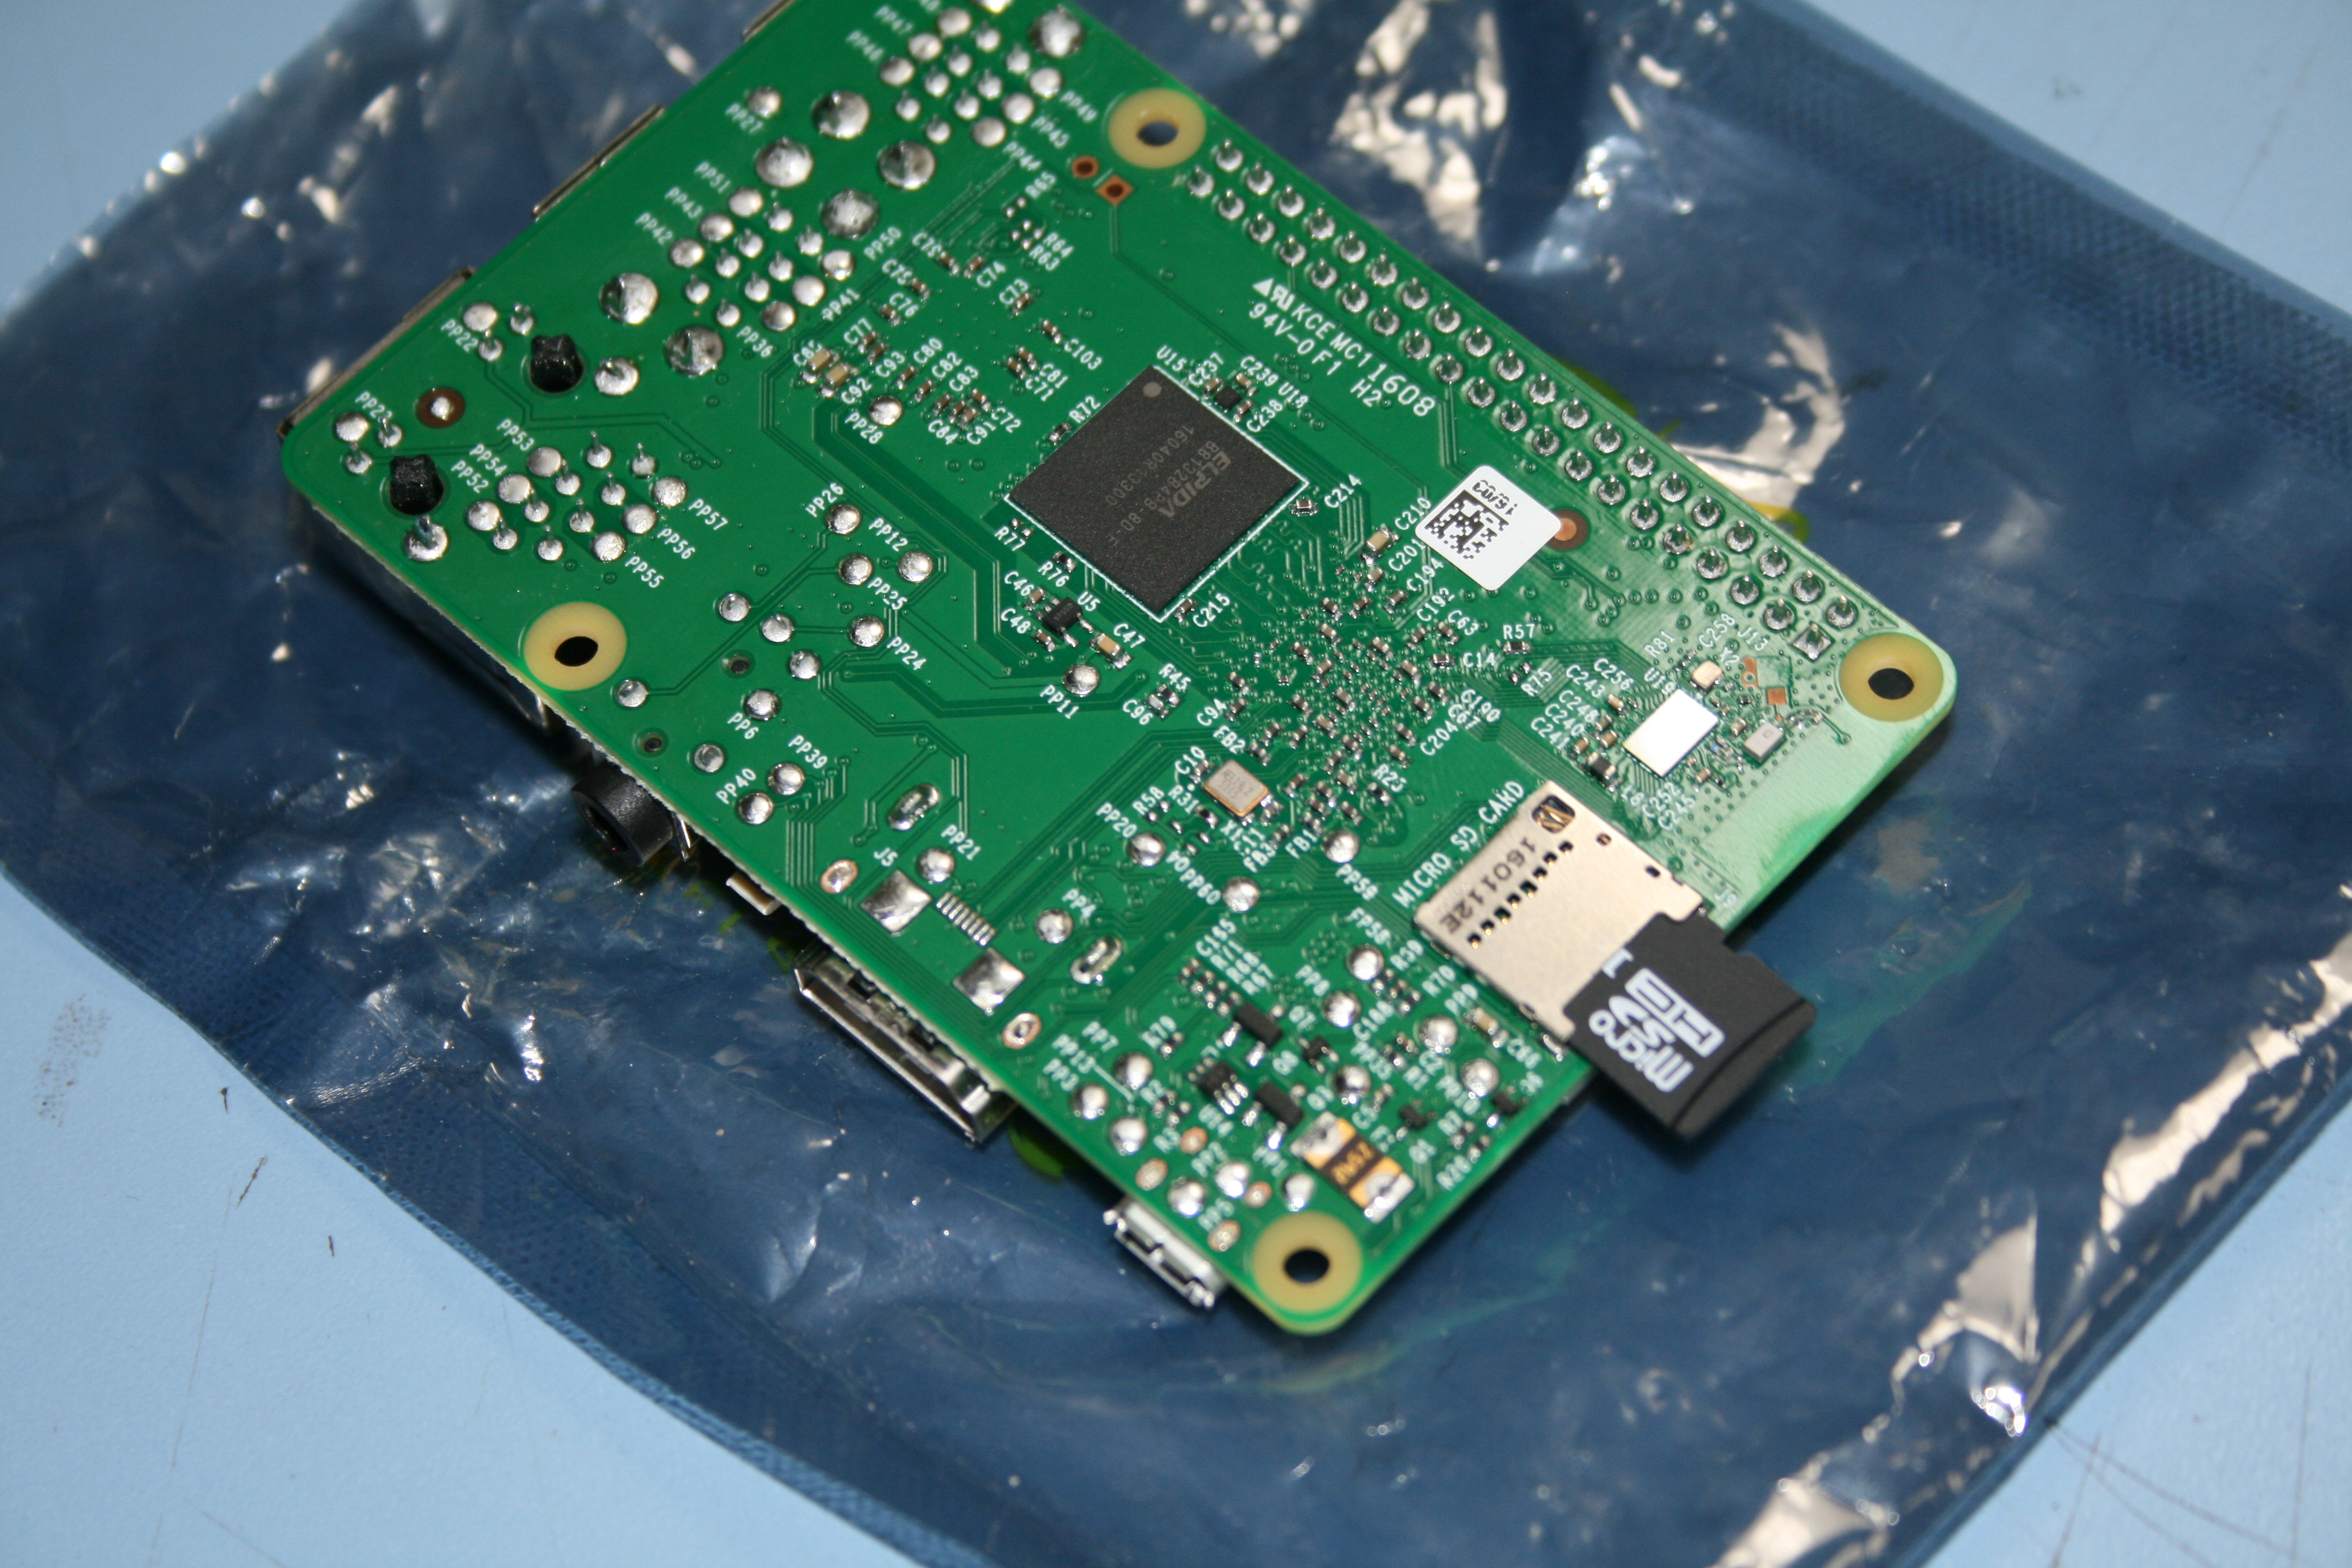
\includegraphics[width=.6\paperwidth]{images/microsd.jpg}}
\end{center}
	\caption{ \textit{La \textit{RaspberryPi} de dos}}
\end{figure}\\

	\item Ensuite, nous allons pouvoir lancer la \textit{RaspberryPi}. Avant de l'alimenter, nous allons distinguer deux cas.. Si vous avez la possibilité, de façon extérieur, d'accéder à l'adresse IP de votre \textit{RaspberryPi} alors vous pouvez sauter l'étape N°3. Si cela n'est pas possible, brancher un écran et un clavier.\\
	Vous pouvez maintenant l'alimenter en utilisant le port micro USB qui est à côté du port HDMI.\\
	
	\item Si vous suivez cette étape, vous devriez voir apparaître des lignes de commandes qui défilent. Quelques instants plus tard, vous arrivez sur l'environnement de bureau de votre \textit{RaspberryPi}.\\
	% faire la demarche pour ouvrir un terminal.
Une fois le terminal ouvert, entrer la commande suivante :\\
\begin{lstlisting}[style=MyBashStyle]
	sudo ifconfig
\end{lstlisting}
un mot de passe devrait vous être demandé, par défaut, le mot de passe est "robots1234"

	\item Très bien, désormais que vous avez l'adresse IP à disposition, nous allons pouvoir installer le nécessaire pour utiliser nos capteurs. Nous aurions très bien pu continuer cette installation directement sur la \textit{RaspberryPi} mais si vous n'avez jamais fait ce qui va suivre, cela vous fera un bon entrainement.\\

\begin{enumerate} 
	\item Télécharger le logiciel \href{https://git-for-windows.github.io/}{Git Bash}
	\item Lancer \textit{Git Bash}
	\item taper la commande en remplaçant "xxx.xxx.xxx.xxx" par l'adresse IP de la \textit{RaspberryPi}\\
	\begin{lstlisting}[style=MyBashStyle]
	ssh pi@xxx.xxx.xxx.xxx
	\end{lstlisting}\\
la première fois, il vous sera demander si vous faites confiante, taper alors "yes" puis sur \textit{Entrée}
	\item Le mot de passe est "robots1234". Si tout c'est bien passé, vous devriez avoir cet aperçu :
	
	\item vous naviguez maintenant dans la \textit{RaspberryPi}. Dans un premier temps, nous allons changer le mot de passe car celui ci est un mot de passe par défaut. Enter la commande :\\
	\begin{lstlisting}[style=MyBashStyle]
	sudo raspi-config
	\end{lstlisting}\\
	un écran bleu devrait apparaître. %insérer image ici et expliquer le chmt mdp et expand
	
	\item Quitter le menu pour revenir au terminal.
	\item Maintenant, nous allons installer GrovePi+ pour pouvoir utiliser le \textit{Shield}. Entrer alors les deux commandes suivantes :\\
	\begin{lstlisting}[style=MyBashStyle]
	sudo curl https://raw.githubusercontent.com/DexterInd
	/Raspbian_For_Robots/master/upd_script/fetch_grovepi.sh | bash
	 
	sudo reboot
	\end{lstlisting}\\
	Votre \textit{RaspberryPi} va redémarrer.
	\item Connecter vous à nouveau en "ssh" comme pour l'étape 4 mais cette fois ci avec votre nouveau mot de passe.
	\item Réaliser alors cette suite de commande une à une. Appuyer sur la touche \textit{Entrée} lorsque l'on vous demande de continuer :
	\begin{lstlisting}[style=MyBashStyle]
	cd /home/pi/Desktop
	sudo git clone https://github.com/DexterInd/GrovePi
	cd /home/pi/Desktop/GrovePi/Script
	sudo chmod +x install.sh
	sudo ./install.sh
	\end{lstlisting}\\
	
	\item Appuyez à nouveau sur \textit{Entrée} une fois arrivé sur cette configuration :
	%insérer image
	\item Au moment où la \textit{RaspberryPi} va redémarrer (vous verrez un "Restart" écrit dans le terminal. Appuyez sur \textit{Ctrl + C} pour empêcher le redémarrage.
	\item Effectuer alors la commande :
	\begin{lstlisting}[style=MyBashSyle]
	sudo shutdown now
	\end{lstlisting}\\
	Elle va alors s'arrêter. Vous pouvez alors la débrancher une fois que vous avez un écran noir.
	\end{enumerate}\\
	
		\item Vous pouvez désormais ajouter le \textit{Shield} sur la \textit{RaspberryPi} Comme ci-dessous \textbf{ATTENTION AU BROCHES UTILISÉES SUR LA PHOTO !}\\
		%inserer photo branchement grovepi
		\item Brancher à nouveau la \textit{RaspberryPi}. Vous devriez avoir une LED qui s'allume sur votre \textit{Shield}
		\item nous allons tester s'il a bien été reconnue, pour cela, connecter vous en "ssh" sur votre \textit{RaspberryPi} (vous devriez savoir le faire maintenant !)
		\item lancer la commande :
		\begin{lstlisting]}[style=MyBashStyle]
		sudo i2cdetect -y 1
		\end{lstlisting}
vous devriez obtenir ce résultat, avec le 04 en première ligne. %ajouter image

\end{enumerate}\\

Voilà, la première mise en route de la \textit{RaspberryPi} est terminé, nous allons maintenant pouvoir nous occuper du code pour la station final.

\section{Installation, configuration et test du code de la station avec ses capteurs.}

	
	
